\documentclass[mathNotesPreamble]{subfiles}
\begin{document}
%\relscale{1.4} %TODO
\section{17.8: Divergence Theorem}

    The Divergence Theorem is the three-dimensional version of the flux form of Green's Theorem. Recall the flux form of Green's Theorem:
    \[\underbrace{\oint\limits_C \mathbf F\cdot \vecn\,ds}_{\textcolor{blue}{\textnormal{flux across }C}}=\iint\limits_R \underbrace{(f_x+g_y)}_{\textcolor{blue}{\textnormal{divergence}}}\,dA.\]
  The above means that the cumulative expansion and contraction throughout $R$ equals the flux across the boundary of $R$. The Divergence Theorem computes the flux over a surface $S$ in $\bbr^3$:
  \vspace*{\stretch{1}}
  \begin{center}
    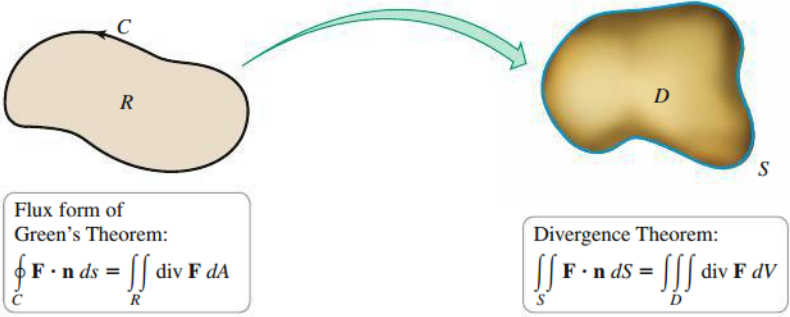
\includegraphics[width=0.75\linewidth]{images/briggs_17_08/fig17_68}
  \end{center}
  \vspace*{\stretch{1}}

  \begin{thmBox*}[Theorem 17.17: Divergence Theorem]
    Let $\mathbf F$ be a vector field whose components have continuous first partial derivatives in a connected and simply connected region $D$ in $\bbr^3$ enclosed by an oriented surface $S$. Then
      \[\iint\limits_S \mathbf F\cdot\vecn\,dS=\iiint\limits_D\grad\cdot\mathbf F\,dV,\]
    where $\vecn$ is the outward unit normal vector on $S$.
  \end{thmBox*}
  \pagebreak

  \begin{ex*}
    \textbf{Verify the Divergence Theorem:} Consider the radial field $\mathbf F=\bracket{x,\,y,\,z}$ and let $S$ be the sphere $x^2+y^2+z^2=a^2$ that encloses the region $D$. Assume $\vecn$ is the outward unit normal vector on the sphere. Evaluate both integrals of the Divergence Theorem.
  \end{ex*}
  \vspace*{\stretch{1}}
  \pagebreak

  \begin{ex*}
    Find the net outward flux of the field $\mathbf F=xyz\bracket{1,1,1}$ across the boundaries of the cube $D=\set{(x,y,z): 0\leq x\leq 1, 0\leq y\leq 1, 0\leq z\leq 1}$.
  \end{ex*}
  \begin{flushright}
    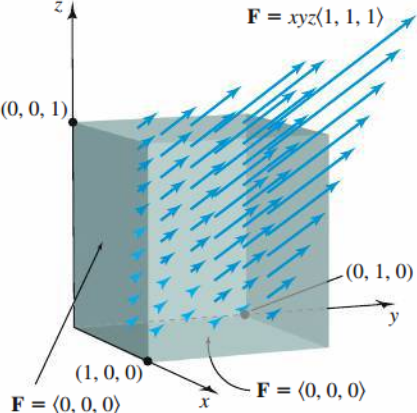
\includegraphics[width=0.35\linewidth]{images/briggs_17_08/fig17_69}
  \end{flushright}
  \vspace*{\stretch{1}}
  \pagebreak

  \begin{thmBox*}[Theorem 17.18: Divergence Theorem for Hollow Regions]
    Suppose the vector field $\mathbf F$ satisfies the conditions of the Divergence Theorem on a region $D$ bounded by two oriented surfaces $S_1$ and $S_2$, where $S_1$ lies within $S_2$. Let $S$ be the entire boundary of $D$ ($S=S_1\cup S_2$) and let $\vecn_1$ and $\vecn_2$ be the outward unit normal vectors for $S_1$ and $S_2$, respectively. Then
      \[\iiint\limits_D \grad\cdot\mathbf F\,dV = \iint\limits_S \mathbf F\cdot\vecn\,dS = \iint\limits_{S_2} \mathbf F\cdot\vecn_2\,dS-\iint\limits_{S_1}\mathbf F\cdot\vecn_2\,dS.\]
  \end{thmBox*}
  \vspace*{\stretch{0.5}}
  \begin{center}
    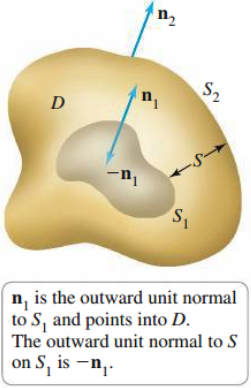
\includegraphics[width=0.3\linewidth]{images/briggs_17_08/fig17_72}
  \end{center}
  \vspace*{\stretch{1}}
  \pagebreak

  \begin{ex*}
    Consider the inverse square vector field
      \[\mathbf F=\frac{\vecr}{\abs{\vecr}^3}=\frac{\bracket{x,\,y,\,z}}{\parens{x^2+y^2+z^2}^{\sfrac{3}{2}}}\]
  \end{ex*}
  \begin{tasks}[after-item-skip=\stretch{1}, label=, item-indent=0pt](1)
    \task Find the net outward flux of $\mathbf F$ across the surface of the region \newline $D=\set{(x,y,z): a^2\leq x^2+y^2+z^2\leq b^2}$ that lies between concentric spheres with radii $a$ and $b$.
    \task 
      Find the outward flux of $\mathbf F$ across any sphere that encloses the origin.
  \end{tasks}
  \vspace*{\stretch{1}}
  \pagebreak

  \begin{ex*}
    Use the Divergence Theorem to compute the net outward flux of the field $\mathbf F=\bracket{x^2,\,y^2,\,z^2}$ across the surface $S$ where $S$ is the sphere $\set{(x,y,z): x^2+y^2+z^2=r^2}$.
  \end{ex*}
  \vspace*{\stretch{1}}
  \pagebreak

  \vspace*{\stretch{1}}
  \begin{center}
    \renewcommand{\arraystretch}{3}
    \begin{tabular}{@{}m{0.32\linewidth}m{0.4\linewidth}m{0.23\linewidth}@{}}\toprule
      \textbf{Fundamental Theorem of Calculus}& $\ds\int_a^b f'(x)\,dx=f(b)-f(a)$& 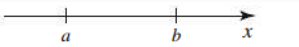
\includegraphics[width=\linewidth]{images/briggs_17_08/tab17_04a}\\
      %
      \textbf{Fundamental Theorem for Line Integrals}& $\ds\int\limits_C \grad f\cdot d\vecr=f(B)-f(A)$& 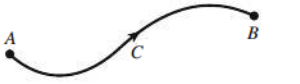
\includegraphics[width=\linewidth]{images/briggs_17_08/tab17_04b}\\
      %
      \textbf{Green's Theorem\newline (Circulation Form)}& $\ds\iint\limits_R \parens{g_x-f_y}\,dA=\oint\limits_C f\,dx+g\,dy$& 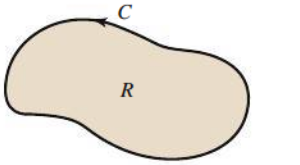
\includegraphics[width=\linewidth]{images/briggs_17_08/tab17_04c}\\
      %
      \textbf{Stokes' Theorem}& $\ds\iint\limits_S \parens{\grad\times\mathbf F}\cdot\vecn\,dS=\oint\limits_C \mathbf F\cdot d\vecr$& 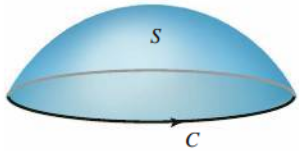
\includegraphics[width=\linewidth]{images/briggs_17_08/tab17_04d}\\
      %
      \textbf{Divergence Theorem}& $\ds\iiint\limits_D \grad\cdot\mathbf F\,dV=\iint\limits_S \mathbf F\cdot\vecn\,dS$& 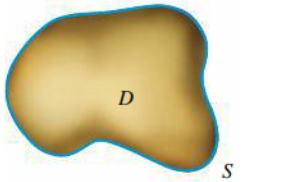
\includegraphics[width=\linewidth]{images/briggs_17_08/tab17_04e}\\\bottomrule
    \end{tabular}
  \end{center}
  \vspace*{\stretch{1}}
  
\end{document}